

This study proposes a dynamic procurement based on machine learning techniques, trained with historical hourly data with custom made model architectures

\subsection{Methodology Implementation}

The methodology applied was a "brute force" choosing of better model, which can lead to better fine tuning results than a more complex architecture as shown in \cite{Liu2022}.\par
With multiple model related variables in study:\par

\begin{table}[H] 
    \caption{Training and architecture variables.\label{training_vars}}
    \newcolumntype{C}{>{\centering\arraybackslash}X}
    \begin{tabularx}{\textwidth}{CC}
    \toprule
    \textbf{Variables} & \textbf{Options} \\
        \midrule
            \multirow[m]{5}{*}{Architecture}	& CNN\\
                                                & LSTM\\
                                                & RNN\\
                                                & UNET\\
                                                & Transformer\\
        \midrule
            \multirow[m]{2}{*}{Advance Loss function}	& Mirror Weights\\
                                                & N/A \\
        \midrule
            \multirow[m]{3}{*}{Loss function}	& \gls{MAE}\\
                                                & \gls{MSE}\\
                                                & \gls{MSLE}\\
        \midrule
            \multirow[m]{3}{*}{Activation}	& linear\\
                                                & relu\\
                                                & gelu\\
        \midrule
            \multirow[m]{3}{*}{Weights}	& Temporal\\
                                                & Distance to mean \\
                                                & No Weights\\    
    \bottomrule
    \end{tabularx}
    % \noindent{\footnotesize{\textsuperscript{1} Tables may have a footer.}}
\end{table}

For that we will study different architectures already proven to work in energy forecast \cite{Costa2022}, or in forecast in general \cite{Hewamalage2021}, such as \gls{FCNN}, \gls{LSTM}, \gls{CNN}. Testing also architectures proven to work in other fields, such as UNET \cite{Shelhamer2014} from image segmentation, or Transformers \cite{Vaswani2017}, the current machine learning state of art architecture. Although for Transformer, processing limitation won't allow for a deep study of potential the given problem.\par
As for the loss function used, we shall test it with the three most common regression loss function: \gls{MAE}, \gls{MSE}, \gls{MSLE}, which are means of the given error, in absolute terms, the square os the errors, and the logarithmic square, respectively. The last two functions give more importance to larger errors.\par
But since the problem we are trying to solve is not only of finding the smallest error, but to make sure the there is less negative and positive error than the benchmark we create a custom loss function to encapsulate the final loss calculation, the Mirror Weights. %\href{https://github.com/alquimodelia/alquitable/blob/main/alquitable/advanced_losses.py#L33}{Mirror Weights}. \par

This function acts as a weight distributor for the negative and positive errors, in such a way that the a ratio defines which size gives more meaning to the final loss calculation. This was created since the error in missing energy is on a $10^{5}$ dimension, and on surplus $10^{6}$.\par
In a default loss function trying to lower the absolute error, this difference means most work would be to lower surplus errors even at the expenses of raising the missing error. The created function allows for more behaviors, and some of them were studied, but the one with better results was defaulting surplus results weight 1, and making the weights of missing values its own error, multiplied by a ratio. Insights on given different ratio outcomes can be seen below:\par


\begin{figure}[H]
    \centering
    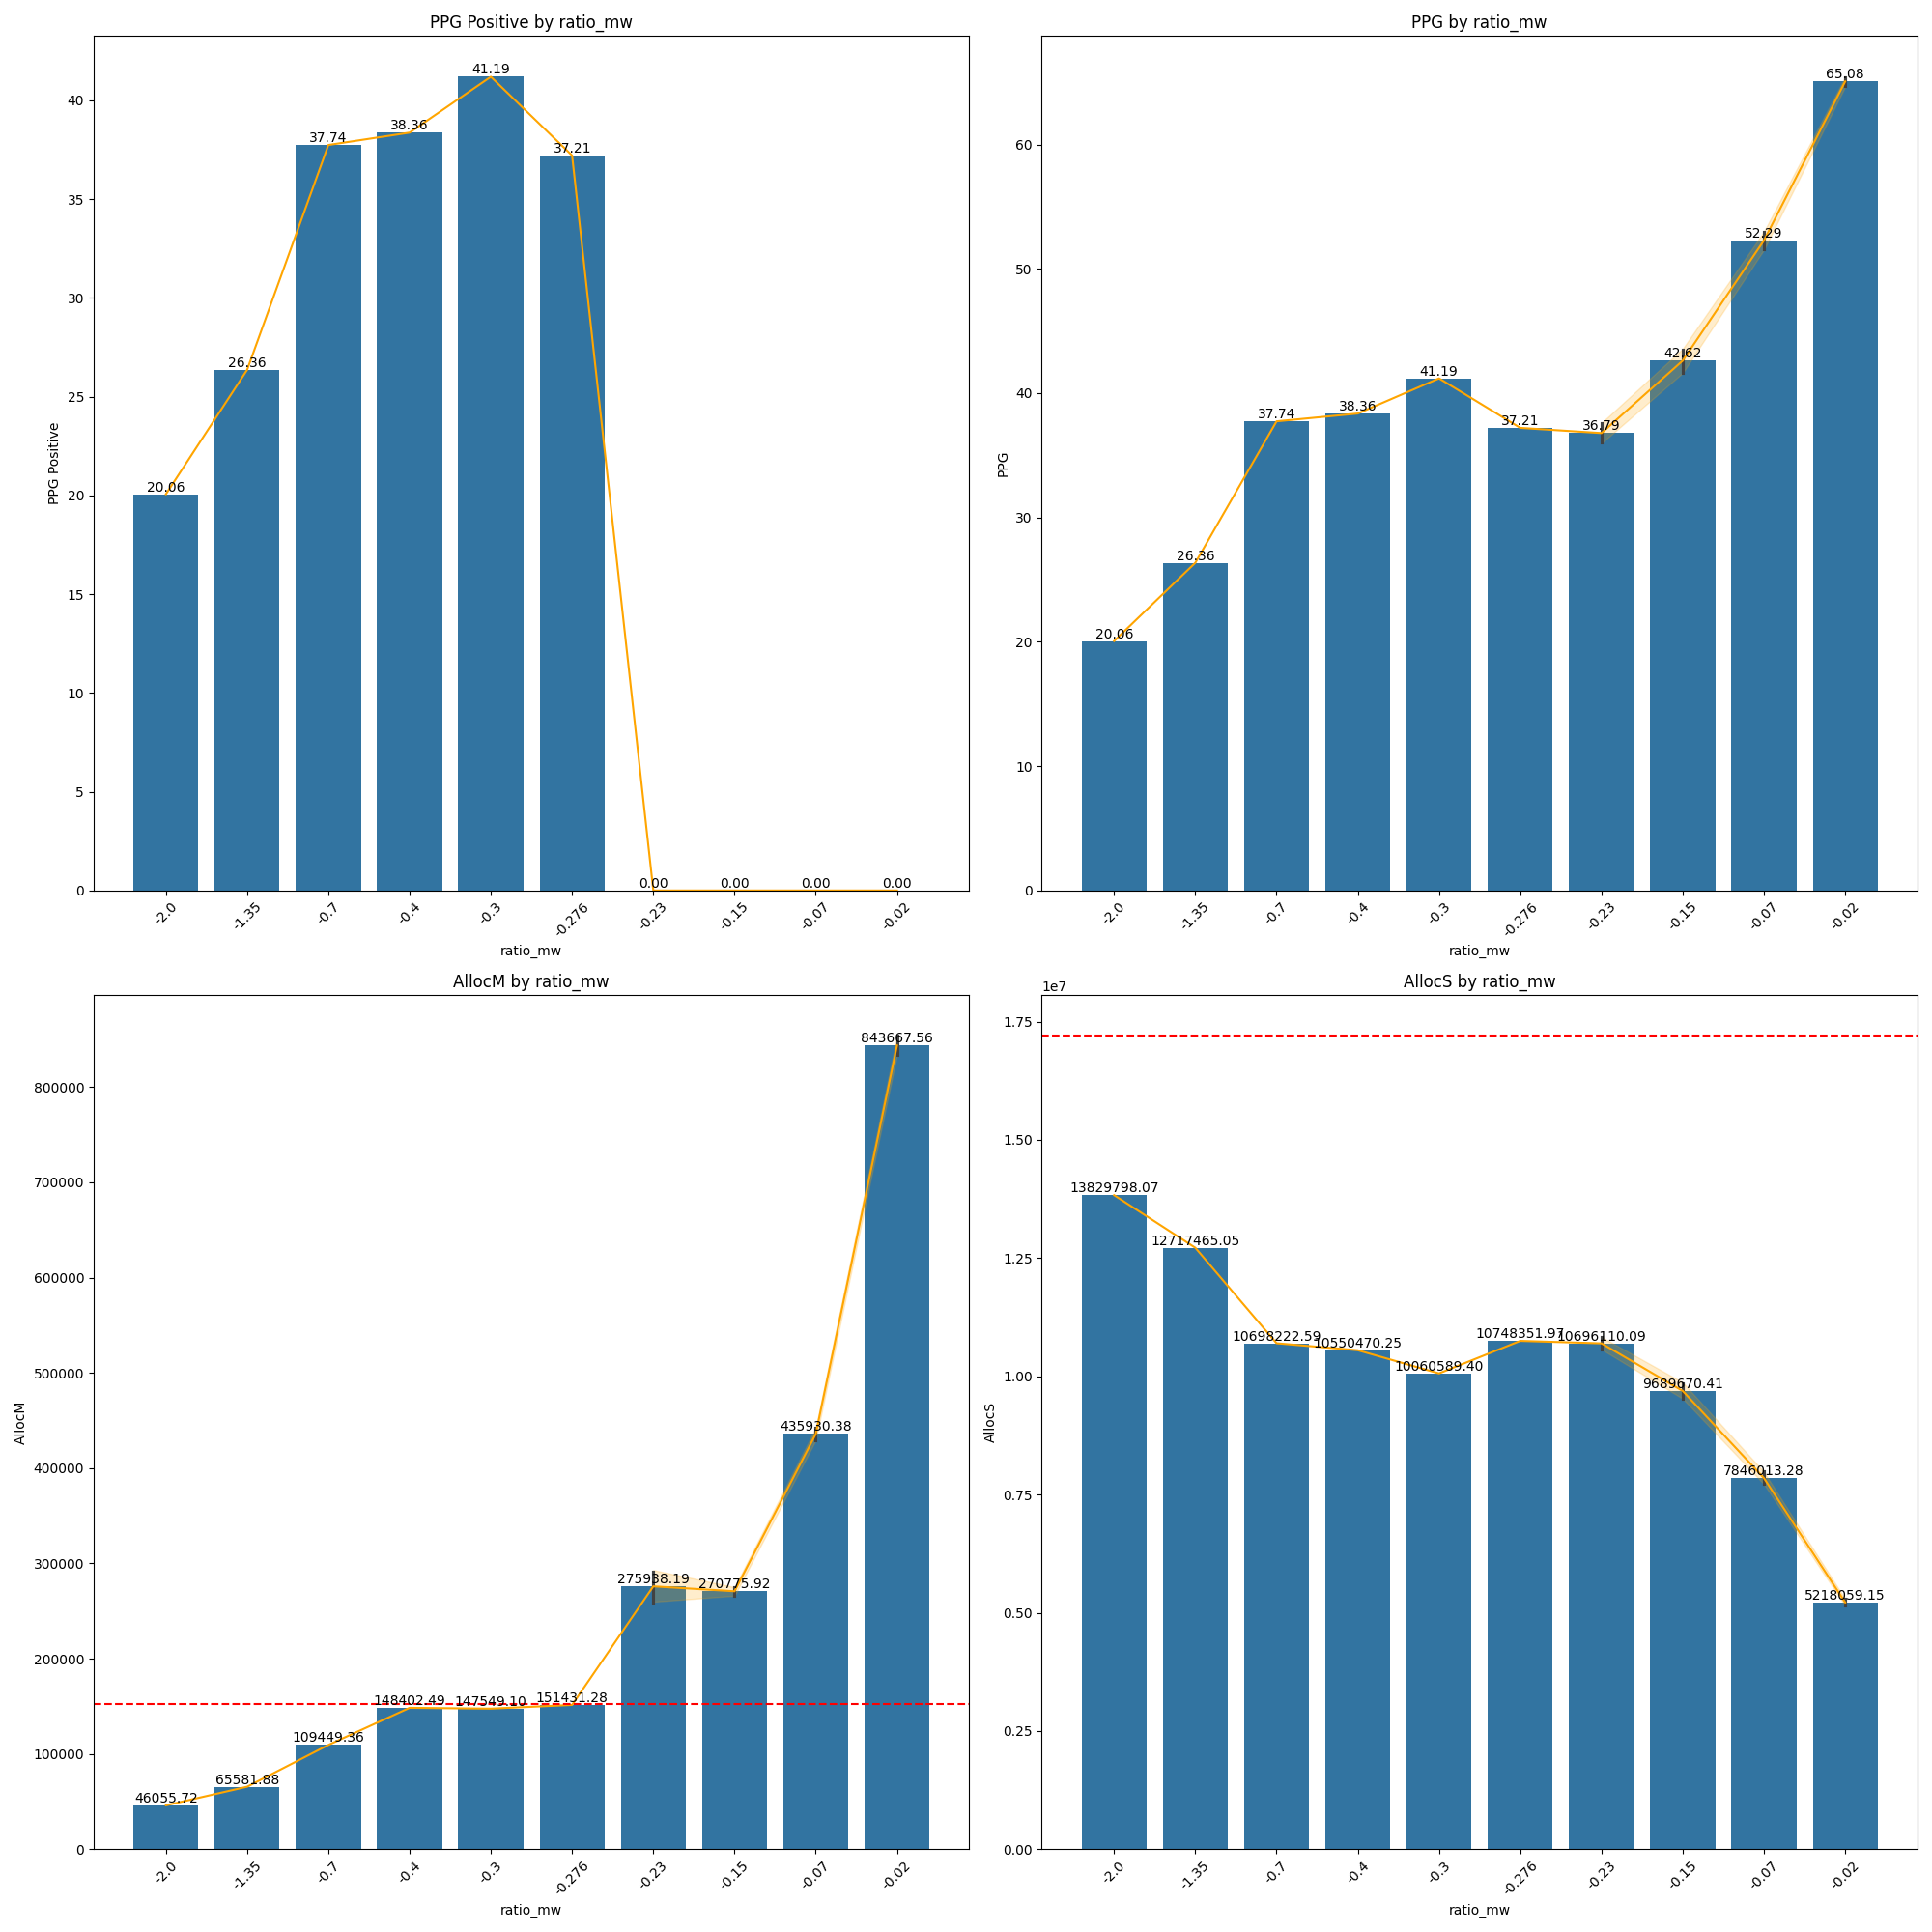
\includegraphics[width=\textwidth]{plots/article_ratio_mw.png}
    \caption{Mirror Weights ratio influence on metrics}
    \label{fig:Ratio_influence_on_metrics}
  \end{figure}
Were the red doted line shows the benchmark values, and our goal is to have both below the benchmark line.\par
As for activation research suggested it could  provide significant impact on the outcome \cite{Vaswani2017,Liu2022}. The test were done using the most common activations for regression problems, where we separated activations inside the model structure (on each deep layer), and the final layer. These are: linear leaves inputs unchanged, \gls{ReLU} outputs the input if positive and zero otherwise, while \gls{GELU} smooth this behavior by applying a Gaussian-based probabilistic transformation. \par
And the last model variable in test were the weights, these given directly to the model training, not in a custom loss function. These weights are multiplied with the Mirror Weights.\par
Temporal weights give weight one to the oldest sample and add one per time sample, making older data less relevant, in an attempt to be more aware of latest trends. The distance to mean purpose is to give more weight values further away from the mean, this would serve as a way to alleviate mean related generalization and catch spike inducing patterns.\par
Where each of the model variables in study is a layer of training, giving the best model within that scope we would go to the next variable with the given best option so far. Going back and forward as to not loose best possible choices.\par


\begin{figure}[H]
	\centering
	\resizebox{\linewidth}{!}{\begin{tikzpicture}[ node distance = 1cm, auto, block/.style={ rectangle, draw, align=center, minimum width=1cm, minimum height=1cm }, line/.style={ draw, -latex' } ]
    % Encoder (Contracting Path)
    \node [block] (archs) {Architectures};
    \node [block,  right=of archs] (advance_loss_function) {Advance Loss Function};
    \node [block,  below=of advance_loss_function] (loss_function) {Loss Functions};
    
    \node[block, fit=(advance_loss_function)(loss_function)] (loss) {};

    
    \node [block,  right=of loss] (activations) {Activations};

    \node [block,  right=of activations] (weights) {Weights};

    % \node [block, below right=of enclayer1, xshift=-1.8cm] (enclayer2) {Enconding2};
    % \node [block, below right=of enclayer2, xshift=-1.6cm] (enclayer3) {Enconding3};
    % % (None, 168, 18) 
    
    % \node [block, below right=of enclayer3] (up1) {Enconding4};
    
    % % Decoder (Expanding Path)
    % \node [block, above right=of up1] (declayer1) {Decoding1};
    % \node [block, above right=of declayer1, xshift=-1.6cm] (declayer2) {Decoding2};
    % \node [block, above right=of declayer2, xshift=-1.8cm] (declayer3) {Decoding3};
    % \node [block, above right=of declayer3, xshift=-2cm] (output) {Output};
    
    % % Skip Connection
    % % \draw [line] (pool1) -- ++(0,-1) -| (up1);
    
    % Connections
    \draw [line] (archs) -- (advance_loss_function);
    \draw [line] (advance_loss_function) -- (loss_function);
    \draw [line] (loss) -- (activations);
    \draw [line] (activations) -- (weights);

    \draw [line, bend right=30] (advance_loss_function) to (archs);



    \draw [line, bend right=30] (weights) to (archs);

    % \draw [line, bend left=30] (loss_function) to (archs);
    % \draw [line] (up1) -- (declayer1);
    
    
    % \draw [line] (declayer1) -- (declayer2);
    % \draw [line] (declayer2) -- (declayer3);
    % \draw [line] (declayer3) -- (output);
    
    
    % \draw [line] (input) -- (output);
    % \draw [line] (enclayer1) -- (declayer3);
    % \draw [line] (enclayer2) -- (declayer2);
    % \draw [line] (enclayer3) -- (declayer1);
    
    
    \end{tikzpicture}}
	\caption{Model choice method scheme.}
	\label{fig:method_training}
\end{figure}

For the purpose of controlling and processing this experiment three python packages were created.

\begin{itemize}
    \item Alquimodelia: A keras based model builder package, to create the necessary models with each different arch and variable.
    \item Alquitable: A keras based workshop package, to create custom callbacks, loss functions, data generators.
    \item MuadDib: A machine learning framework that uses Alquimodelia to test and choose best models on given conditions automatically.
\end{itemize}

The experiments were done using keras>=3 with a torch backend on a CPU laptop. \colorbox[rgb]{1,1,0}{Explicar o que é keras?}

% \subsubsection{Advance Loss Function}


% Para escolher a melhor maneira de distribuir pesos foi criada uma função de perda com diferentes regras, que distribuem o peso da amostra:
% \href{https://github.com/alquimodelia/alquitable/blob/main/alquitable/advanced_losses.py#L33}{Mirror Weights (Pesos Espelhados)},
% que vai distribuir os pesos da amostra consoante um rácio predefinido e o próprio erro da amostra.\par
% Os pesos nas amostras vão ser divididos entre os erros negativos (alocação em demasia) e os positivos (alocação em falta). Consoante uma variável lógica,  uns terão peso 1 e os outros serão o próprio erro em absoluto. Dando assim um peso equivalente ao erro, quanto maior o erro maior o peso da amostra na função de perda, do lado da amostra escolhido (em demasia ou em falta).\par
% O rácio pode ser multiplicado um rácio tanto a um dos pesos como a outro, sendo estes rácios que irão equilibrar as diferenças entre a alocação em falta e a em demasia. Refira-se que o sinal do rácio influencia qual o lado a ser multiplicado.\par
% Este pesos são passados directamente à função de perda em uso.\par


% \begin{figure}[H]
%     \centering
%     \includegraphics[width=\textwidth]{plots/ratio_mw.png}
%     \caption{Resultados de alocações totais em diferentes rácios}
%     \label{fig:resexpratiomw}
%   \end{figure}

% Estas variações no rácio produzem diferentes dimensões nas alocações, modificando assim a sua posição em relação ao \textit{benchmark}. Aqui para cada arquitetura o rácio ideal para o melhor GPD Positivo diferencia ligeiramente, tendo sido procurado com tentativa/erro baseado em assunções perante a aparente distribuição rácio/alocações.\par


\subsection{Metrics}

With distinct weights, the metrics, are used to choose best model on each iteration, and they can be divided into two groups:

\begin{enumerate}
\item Model metrics, where we just use the usual regression metrics adding a metric for how much did the model missed in allocating for the validation period.
\item Comparative metrics, where we assert percentage gains over the current allocation method. 
\end{enumerate} 

\subsubsection{Model Metrics}
\begin{linenomath}
    \begin{equation}\label{eq:rmse}
        RMSE = \sqrt{\frac{1}{n} \sum_{i=1}^{n}(t_i - p_i)^2}
    \end{equation}
    \end{linenomath}
		
		where $t$ is the observed value, $p$ is the forecast and $n$ is the number of samples.

\begin{linenomath}
    \begin{equation}\label{eq:SAE}
        SAE = \sum_{i=1}^{n}\left|t_i - p_i \right|
    \end{equation}
    \end{linenomath}

SAE can be divide into the following metrics, where we obtain the error, within the time period, of allocated energy not enough for the needs, and too much energy allocated, separately.\\

The \gls{AllocM} is computed as follows:
\begin{linenomath}
    \begin{equation}\label{eq:AllocM}
        AllocM = \sum_{i=1}^{n}\left|t_i - p_i \right| , \text{if } p_i < t_i
        \end{equation}
    \end{linenomath}

The \gls{AllocS} is computed as follows:

\begin{linenomath}
    \begin{equation}\label{eq:AllocS}
        AllocS = \sum_{i=1}^{n}\left|t_i - p_i \right| , \text{if } p_i > t_i
            \end{equation}
    \end{linenomath}
		
These metrics are needed to get a better error than the benchmark, but also to have less wasted \gls{AllocM}, and less occurrences of \gls{AllocS}.\par

\subsubsection{Model/benchmark comparative metrics}

\gls{PPG} is the percentage of how much better is the model over the benchmark, it is computed as follows: 
\begin{linenomath}
    \begin{equation}\label{eq:PPG}
        PPG = \frac{SAE_{benchmark} - SAE_{modelo}}{SAE_{benchmark}} \times 100
    \end{equation}
    \end{linenomath}
		
The following metrics are the same but for only missing allocation and surplus allocation.\\
\gls{PPGM} computes the performance of the missing allocation as follows:\\

\begin{linenomath}
    \begin{equation}\label{eq:PPGM}
        PPGM = \frac{AllocM_{benchmark} - AllocM_{modelo}}{AllocM_{benchmark}} \times 100
    \end{equation}
    \end{linenomath}
		
\gls{PPGM} computes the performance of the surplus allocation as follows:

\begin{linenomath}
    \begin{equation}\label{eq:PPGS}
        PPGS = \frac{AllocS_{benchmark} - AllocS_{modelo}}{AllocS_{benchmark}} \times 100
    \end{equation}
    \end{linenomath}

The \gls{PPG}Positive metric is showing how much better is the model over the benchmark, but only if \gls{PPGM} and \gls{PPGM} are positive.\\

\begin{linenomath}
    \begin{equation}\label{eq:PPGPositive}
        PPG Positive = 
        \begin{cases} 
            PPG & , \text{if } PPGM \text{ }\&\text{ } PPGS \geq 0 \\
            0 & , \text{if } PPGM \text{ }\|\text{ } PPGS < 0 \\
        \end{cases} 
        \end{equation}
    \end{linenomath}



% To address the challenges introduced by \gls{vRES}, dynamic reserve procurement methods have been proposed. Unlike static methods, dynamic approaches consider real-time or near real-time forecasts of energy demand and renewable generation, allowing \gls{TSO}s to adjust reserve allocations accordingly. This adaptability reduces over-procurement and minimizes costs, improving the efficiency of reserve markets.

% The adoption of advanced forecasting tools, particularly machine learning techniques, is central to enabling dynamic reserve procurement. By leveraging historical and operational data, machine learning models can predict reserve needs with greater accuracy, addressing the uncertainties associated with \gls{vRES} generation. Studies have shown that these models outperform traditional statistical methods, offering significant improvements in reserve management and cost reduction.

% In conclusion, the evolving electricity markets and ancillary services frameworks must adapt to the challenges posed by high \gls{vRES} penetration. Dynamic reserve procurement, supported by advanced forecasting techniques and market design improvements, offers a path toward more efficient and reliable power systems.


% The dynamic procurement of secondary reserves represents a significant step forward in addressing the inefficiencies inherent in traditional static allocation methods. Unlike static reserve procurement, which relies on fixed ratios or historical averages, dynamic approaches incorporate real-time forecasts and system conditions to adjust reserve requirements. This adaptability is particularly critical for modern electricity systems with high penetration of \gls{vRES}, where forecasting uncertainty and rapid changes in generation output challenge grid stability.

% Dynamic reserve procurement involves estimating upward and downward reserve needs based on the expected deviations between day-ahead scheduled generation and real-time demand. By leveraging advanced forecasting tools, such as machine learning models, it becomes possible to predict these deviations with greater accuracy, optimizing the allocation of secondary reserves. Historical data on vRES production, system demand, and grid imbalances serve as inputs to these models, allowing the identification of patterns and trends that inform reserve procurement decisions.

% Machine learning techniques, including \gls{LSTM} networks and other time-series forecasting models, have demonstrated significant potential for improving reserve predictions \cite{Costa2022}\cite{Benti2023}. These models can capture the nonlinear and temporal dependencies present in renewable energy data, outperforming traditional statistical methods such as ARIMA. By incorporating real-time weather forecasts, generation data, and demand profiles, dynamic approaches ensure that reserve procurement aligns more closely with actual system needs, reducing both over-procurement and under-procurement of reserves.

% The dynamic approach also allows for asymmetrical procurement of upward and downward reserves, which is particularly relevant in systems with variable renewable generation. For instance, during periods of high solar generation, upward reserves may be less critical, whereas downward reserves become essential to accommodate excess production. Conversely, during low renewable output, upward reserves are prioritized to address potential generation shortfalls.

% In summary, dynamic procurement of secondary reserves offers a more efficient and adaptive solution to balancing challenges in modern electricity systems. By leveraging machine learning techniques and real-time forecasts, this approach enhances reserve allocation, reduces operational costs, improving penetration of \gls{vRES}.

% % \section{Contextualização e motivação do trabalho\label{ch:contextos}}

% \subsection{Mercados de Energia}

% \subsubsection{Mercado Ibérico de Electricidade \label{se:mibel}}

% O \gls{MIBEL} é um exemplo de integração de mercados de energia entre países, funcionando como um elo entre os mercados de eletricidade de Portugal, \gls{OMIP} e Espanha, \gls{OMIE}. Este mercado grossista compreende diferentes formatos de negociação, cada um desempenhando um papel específico na gestão da compra e venda de eletricidade.\par
% O \gls{OMIP} é responsável pela negociação a prazo de energia elétrica, enquanto que o \gls{OMIE} é responsável pela negociação diária de energia elétrica.\par
% O \gls{MIBEL} é estruturado para fornecer uma plataforma eficiente e transparente para a transação de energia, garantindo a competitividade e a segurança de fornecimento. De seguida, vamos propomo-nos a explorar os principais componentes deste modelo:\par


% \paragraph{Mercado em Bolsa (Mercado Spot) \label{se:mercado_bolsa}}
% \text{ }  \par
% O mercado em bolsa, também conhecido como mercado \textit{spot}, é uma das principais formas de negociação no \gls{MIBEL}. Este mercado encontra-se dividido em duas vertentes: o mercado diário e o mercado intradiário. No mercado diário, as propostas de compra e venda de eletricidade são apresentadas para o dia seguinte, permitindo que os agentes ajustem as suas previsões de produção e consumo com base nas condições de mercado mais recentes. Já o mercado intradiário permite a negociação para as horas seguintes, oferecendo maior flexibilidade para ajustes de última hora, o que é especialmente útil para acomodar variações inesperadas na oferta e procura. Este sistema dinâmico assegura que a eletricidade é negociada perto do tempo real, refletindo, assim, as necessidades e capacidades do sistema elétrico com um horizonte a curto prazo.\par


% \paragraph{Mercado de Contratação a Prazo \label{se:mercado_prazo}}
% \text{ }  \par
% Além do mercado \textit{spot}, o \gls{MIBEL} inclui o mercado de contratação a prazo, onde os agentes estipulam compromissos de compra e venda de eletricidade com semanas, meses, ou até anos de antecedência. Este mercado permite aos participantes fixar preços e volumes de energia para o futuro, mitigando os riscos associados à volatilidade dos preços no curto prazo. A contratação a prazo proporciona uma maior previsibilidade e estabilidade financeira para os produtores e consumidores de energia, permitindo um planeamento estratégico mais robusto. Os contratos podem variar em termos de longevidade, desde acordos de curto prazo até contratos a longo prazo, dependendo das necessidades e estratégias dos agentes envolvidos.\par


% \paragraph{Mercado Livre de Contratação Bilateral Física \label{se:mercado_bilateral}}
% \text{ }  \par
% Outra componente importante do \gls{MIBEL} é o mercado livre de contratação bilateral física, onde os agentes negociam diretamente a compra e venda de eletricidade para um determinado período no futuro. Este formato permite uma maior personalização dos contratos, uma vez que as condições podem ser ajustadas diretamente entre as partes envolvidas, sem a intervenção de um mercado centralizado. Esse tipo de negociação é particularmente vantajoso para grandes consumidores e produtores que procuram acordos específicos para atender às suas necessidades operacionais ou estratégias de \textit{hedging} (mitigação de risco) contra flutuações de preços. A liberdade de negociação bilateral física oferece um nível adicional de flexibilidade e controlo sobre as transações, promovendo uma maior eficiência no mercado.\par

% \paragraph{Mercado de Serviços de Sistema \label{se:servicos_sistema_mibel}}
% \text{ }  \par
% Por fim, o mercado de serviços de sistema desempenha um papel crítico na manutenção do equilíbrio entre a produção e o consumo de energia elétrica em tempo real. Este mercado é responsável por garantir que a rede elétrica opere de forma segura e estável, ativando reservas e ajustando a produção conforme necessário para responder a variações inesperadas na procura ou na oferta. O mercado de serviços de sistema engloba uma série de mecanismos, incluindo a ativação de reservas de frequência e o despacho de unidades geradoras flexíveis, que são essenciais para a gestão da estabilidade da rede. A participação neste mercado é muitas vezes obrigatória para certos tipos de geradores, especialmente aqueles que possuem a capacidade de resposta rápida, como hidroelétricas e centrais térmicas.\par
% Os mercados de serviços de sistema, português e espanhol, são geridos independentemente, onde o \gls{GGS} é o operador do mercado no respectivo país, sendo a \gls{REN} em Portugal e a \gls{REE} em Espanha.\par
% \bigskip
% \bigskip
% Sumariamente, o \gls{MIBEL} é um mercado complexo e multifacetado que oferece uma ampla gama de formatos de negociação para atender às diversas necessidades dos agentes de mercado. Desde a negociação em tempo real no mercado \textit{spot} até compromissos de longo prazo no mercado de contratação a prazo e acordos personalizados no mercado bilateral, o \gls{MIBEL} proporciona um ambiente robusto para a transação de eletricidade, promovendo a eficiência, a flexibilidade e a segurança do fornecimento de energia na Península Ibérica.\cite{Rassid2017}\par



% \begin{figure}[H]
% 	\centering
% 	\resizebox{\linewidth}{!}{\begin{tikzpicture} [ node distance = 1cm, auto, block/.style={ rectangle, draw, align=center, minimum width=2cm, minimum height=1cm }, line/.style={ draw, -latex' } ]

    \node [block] (top) {Mercados Organizados};
    \node [block, below=of top](spot) {Mercado Spot \gls{OMIE}}; 

    \node [block, left=of spot](prazo) {Contractos a prazo \gls{OMIP}}; 
    \node [block, right=of spot](ss) {Serviços de Sistema};

    \draw [line] (top) -| (prazo);
    \draw [line] (top) -- (spot);
    \draw [line] (top) -| (ss);
    
    \node[fit=(top)(spot)(prazo)(ss)] (group) {};

    \node[block, left=of group, minimum width=1cm, minimum height=4cm] (left_block) {Contractos Bilaterais};

    \node[fit=(left_block)(prazo)(spot)] (group2) {};

    \path let \p1 = (left_block.west), \p2 = (spot.east) in
        node [block, below=of group2, minimum width={\x2-\x1}] (group2) {Negociação Mibel};


    \node[block, below right=of ss, xshift=-1cm] (ren) {Portugal \gls{REN}};
    \node[block, below=of ren] (ree) {Espanha \gls{REE}};
    \draw [line] (ss) |- (ren);
    \draw [line] (ss) |- (ree);


    \end{tikzpicture}}
% 	\caption{Organizaçao MIBEL. Adaptado de \cite{Rassid2017}}
% 	\label{fig:mibel_org}
% \end{figure}




% \subsubsection{Mercado de Serviços de Sistema \label{se:servicos_sistema}}

% % \paragraph{Introdução ao Mercado de Serviços de Sistema \label{se:intro_servicos_sistema}}
% % \text{ }  \par

% O mercado de serviços de sistema é uma componente fundamental dos mercados de energia, desempenhando um papel crucial na manutenção da segurança e estabilidade das redes elétricas \cite{dgegmss}. Esses serviços são essenciais para garantir que a produção e o consumo de energia permaneçam em equilíbrio, um requisito vital para o funcionamento seguro e eficiente de qualquer sistema eléctrico. A principal função dos serviços de sistema é assegurar a qualidade da energia fornecida, monitorizando parâmetros críticos como a frequência, a potência activa e reactiva, controlando a tensão na rede, arranque automático e outras técnicas de sistemas. Esse controlo é realizado através da coordenação entre os geradores e os consumidores, com o objetivo de responder rapidamente a variações na oferta e na procura de energia \cite{Rassid2017} \cite{Carneiro2016}.\par
% No contexto europeu, a regulação desses serviços é coordenada pela \gls{ENTSO-E}, que estabelece os requisitos e normas para a operação dos sistemas de energia, e a operação dos mesmos é da responsabilidade dos \gls{TSO} nacionais. Essas reservas são activadas conforme necessário para manter a frequência da rede no seu valor nominal de 50Hz, ajustando a potência activa dos geradores em resposta a variações imprevistas na procura ou na oferta de energia.\par
% As reservas de frequência,ou reservas de controlo, são divididas em três categorias principais: primária, \gls{FCR}, secundária, \gls{aFRR}, e terciária, \gls{mFRR}, cada uma com funções específicas e tempos de resposta distintos. A reserva primária é activada automaticamente e de forma quase instantânea, dentro de segundos após um distúrbio na rede, para estabilizar rapidamente a frequência. A reserva secundária entra em ação logo em seguida, substituindo gradualmente a reserva primária e ajustando a frequência de volta ao seu valor programado. Finalmente, a reserva terciária é utilizada para corrigir desvios de longo prazo e libertar as outras reservas para possíveis eventos futuros, completando o ciclo de controlo da frequência e assegurando que o sistema retorne a um estado de equilíbrio estável.\par
% Todas estas correções no sistema podem ser efectuadas tanto a injectar mais potência na rede, como a diminuir a potência existente, a estas chamamos Banda a Subir e Banda a Descer, respectivamente.\par
% A harmonização dos mercados europeus de eletricidade, especialmente nos mercados diários, intradiários e de balanço, é uma realidade em desenvolvimento que procura reduzir custos e melhorar as condições de participação para todos os envolvidos \cite{Algarvio2019}. No entanto, a integração das \gls{vRES}, como a eólica e a solar, apresenta desafios adicionais devido à sua natureza intermitente e dependente de condições climáticas. Embora tecnicamente viável, devido a este paradigma de imprevisibilidade e ao facto de serem fontes não despacháveis, a participação dessas fontes nos mercados de balanço enfrenta restrições significativas para garantir a segurança e a estabilidade da rede.\par
% A actual infraestrutura dos mercados de serviços de sistema precisa, portanto, de ser adaptada para acomodar essas novas fontes de energia. Uma parte essencial dessa adaptação é o desenvolvimento de métodos mais robustos para prever a necessidade de reservas, que tenham em consideração a variabilidade das \gls{vRES}. Actualmente, as previsões são baseadas principalmente em fórmulas criadas pelas operadoras, mas esta abordagem muitas vezes falha em capturar a complexidade e a incerteza associadas à produção renovável. Assim, há uma crescente exploração de técnicas avançadas, como o uso de modelos de \textit{machine learning}, para melhorar a precisão das previsões e otimizar a gestão das reservas.
% Além disso, a evolução para um mercado pan-europeu harmonizado de serviços de sistema envolve não apenas a uniformização de regras e requisitos técnicos, mas também a criação de incentivos económicos que tornem a participação atraente para todos os tipos de produtores de energia, incluindo os renováveis. Isso é particularmente importante, uma vez que os mercados de balanço são fundamentais para garantir que as redes elétricas possam operar de forma estável e segura, mesmo com altas penetrações de \gls{vRES}. Ao permitir que essas fontes renováveis participem de forma mais activa e competitiva nos mercados de balanço, espera-se não apenas reduzir os custos de operação dos sistemas eléctricos, mas também aumentar a viabilidade económica das \gls{vRES}.\par
% Com a crescente dependência de fontes de energia renovável e a necessidade de sistemas eléctricos mais resilientes e flexíveis, o papel dos serviços de sistema continuará a expandir-se e a evoluir, exigindo inovações tanto na gestão técnica como na regulação económica dos mercados de energia.\par


% \paragraph{Estrutura e Funcionamento das Reservas de Frequência \label{se:reservas_freq}}
% \text{ }  \par


% A reserva primária, \gls{FCR}, é o primeiro nível de resposta e é accionada automaticamente em questão de segundos após a detecção de um desvio de frequência, que pode ocorrer devido a falhas na produção ou variações repentinas na procura. Esta reserva é activada até 15 segundos após o distúrbio e permanece activa por cerca de 30 segundos, ou até que a reserva secundária possa assumir o controlo. A \gls{FCR} é geralmente suportada por geradores que possuem capacidade técnica para resposta rápida, como hidroelétricas e algumas unidades térmicas. Este serviço é obrigatório para todos os geradores conectados à rede que possuem a capacidade técnica necessária, e não é remunerado em muitos mercados europeus, incluindo o mercado ibérico.\par
% A reserva secundária, \gls{aFRR}, entra em ação logo após a activação da reserva primária, com o objetivo de restaurar a frequência da rede ao seu valor programado de 50 Hz e libertar a \gls{FCR} para responder a possíveis distúrbios subsequentes. A \gls{aFRR} é activada automaticamente até 30 segundos após o desvio inicial e pode levar até 15 minutos para corrigir completamente o desequilíbrio. Este tipo de reserva é contratado em mercados específicos de banda de reserva, nos quais os geradores submetem ofertas para fornecer a capacidade necessária.\par
% A reserva terciária, \gls{mFRR}, é o último nível de resposta e é utilizada principalmente para corrigir desequilíbrios de longo prazo e libertar a \gls{aFRR} para outros usos. Ao contrário das reservas primária e secundária, a \gls{mFRR} é activada manualmente pelos \gls{TSO} e pode levar até 15 minutos a estar completamente activa. Esta reserva é frequentemente utilizada para ajustar a geração ou o consumo de energia de acordo com desvios significativos e prolongados, que não podem ser compensados de forma eficaz pelas reservas de resposta mais rápida. A \gls{mFRR} é geralmente suportada por geradores que podem oferecer flexibilidade nas operações, como algumas centrais térmicas e hidroelétricas de grande dimensão.\par

% Este esquema pode ser representado pela seguinte figura:\par
% \begin{figure}[H]
%   \centering
%   \includegraphics[width=\textwidth]{../../dissertation/plots/actiavtion_example.png}
%   \caption{Esquema de activação do sistema de reservas. Adaptado de \cite{handbook2009policy}}
%   \label{fig:targettimeserieswindows}
% \end{figure}

\subsection{Previsão de Necessidades de Reservas \label{se:pred_impact_vres}}

A previsão das necessidades de reservas de frequência é uma componente essencial na gestão eficiente dos sistemas eléctricos, especialmente num cenário de crescente penetração das \gls{vRES}.\par
O uso de técnicas de \textit{machine learning} tem sido explorado como uma solução promissora para melhorar essas previsões. Estes modelos podem analisar grandes volumes de dados, identificar padrões complexos e ajustar previsões em tempo real, considerando factores como mudanças nas condições meteorológicas e padrões de consumo de energia. Ao incorporar a variabilidade das \gls{vRES} nos modelos de previsão, é possível reduzir a incerteza e melhorar a alocação das reservas de frequência, resultando numa operação mais eficiente do sistema eléctrico.\par
Outro factor crítico na previsão das necessidades de reservas de frequência é a coordenação entre diferentes mercados e operadores de sistemas. A harmonização dos mercados europeus de balanço, incluindo a padronização das regras de oferta, leilão e remuneração, pode facilitar a integração das \gls{vRES} e melhorar a eficiência geral do sistema. Com regras claras e uniformes, os produtores de energia renovável têm maior incentivo para participar activamente dos mercados de reservas, fornecendo capacidade adicional para apoiar a estabilidade da rede. Esta questão é particularmente relevante em mercados onde as \gls{vRES} ainda enfrentam barreiras significativas para a participação, como regras complexas de licitação ou altos requisitos de capacidade mínima para participação.\par
Apesar dos avanços na previsão de necessidades de reservas, ainda existem desafios consideráveis. A precisão das previsões pode ser limitada pela qualidade dos dados disponíveis, bem como pela capacidade dos modelos de capturar todas as variáveis relevantes que afetam a operação da rede. Além disso, a crescente interconexão dos sistemas eléctricos e o aumento da troca de energia entre países exigem uma abordagem coordenada e colaborativa para a previsão de reservas, considerando tanto as condições locais como as condições regionais.\par
O desenvolvimento contínuo de técnicas avançadas de previsão e a integração de soluções baseadas em dados serão fundamentais para enfrentar esses desafios. À medida que mais dados históricos se tornam disponíveis e os modelos de previsão evoluem, espera-se que a gestão das reservas de frequência se torne cada vez mais eficiente, contribuindo para um sistema eléctrico mais resiliente e capaz de integrar altos níveis de Tal desenvolvimento, não apenas reduzirá os custos operacionais, mas também contribuirá para a segurança energética e para a transição para um sistema energético mais sustentável.\par

\subsubsection{Previsão de Banda Secundária no Mercado Ibérico de Electricidade \label{se:pred_mibel}}
A nível Europeu a \gls{ENTSO-E} providencia várias metodologias para o dimensionamento das reservas de controlo descritas em \cite{handbook2009policy}. A quantidade mínima recomendada de alocação necessária para a reserva de controlo secundária pode ser descrita da seguinte forma:\par

\begin{equation} \label{eq:BRENTSOE} 
    BR = \sqrt{a \times  L_{max} + b^{2}} - b 
\end{equation}
onde:
\begin{itemize}
  \item $BR$: Banda de Reserva de regulação secundária mínima necessária (MW).
  \item $a$ e $b$: Coeficientes empiricos, $a$=10MW e $b$=150MW .
  \item $L_{max}$: Consumo máximo antecipado (MW).
\end{itemize}


\paragraph{Portugal \label{se:prev_portugal}}
\text{ }  \par

No mercado português para dimensionar a \gls{aFRR} a \gls{REN} utiliza por base a equação \ref{eq:BRENTSOE} multiplicando um parâmetro horário, $\rho$:

\begin{equation} \label{eq:BRREN} 
    BR = \rho \times \sqrt{a \times  L_{max} + b^{2}} - b 
\end{equation}
onde:
\begin{itemize}
  \item $\rho$: Paramêtro horário.
\end{itemize}


Na equação \ref{eq:BRREN} BR equivale à banda a subir, sendo a banda a descer metade da banda a subir. De notar que em \cite{Carneiro2016} BR é a banda de reserva, que equivale à soma da banda a subir e banda a descer, onde aí é sempre considerado que banda a subir são $\frac{2}{3}$ da Banda de Reserva total e a banda a descer é o restante $\frac{1}{3}$.\par
Este método de cálculo permite manter as reservas a corresponder às necessidades do sistema, mas têm uma uma alocação  em excesso. Podemos verificar que no período 2013 a 2023, inclusive, as médias por hora têm cerca de 437\% de alocação em excesso, o que corresponde, em média, a cerca de 221 MWh desperdiçados a cada hora. \par

\begin{table}[H]
	\centering
    \caption{Média das Bandas Alocada e Usada (REN)}    
    \resizebox{!}{!}{\begin{tabular}{rrrr}
\toprule
Banda de Reserva Alocada & Banda Reserva Activada & erro & erro \% \\
\midrule
271.57 & 50.53 & 221.04 & 437.43 \\
\bottomrule
\end{tabular}
}
    \label{tab:media_bandas_pt}
    \end{table}

Estando actualmente o \gls{TSO} português a utilizar esta fórmula, e a obter estes resultados, este é um bom caso de estudo de optimização dos parâmetros da fórmula. Sendo que \textit{a} e \textit{b} são dados pela entidade europeia, propõe-se o estudo do parâmetro horário de modo a corresponder a banda de reserva calculada ao consumo real.\par

\paragraph{Espanha \label{se:prev_espanha}}
\text{ }  \par

No mercado espanhol não encontramos directivas de uso de uma fórmula como no caso português. Nem encontramos uma simetria directa entre as bandas a subir e a descer. Contudo, podemos verificar que a média horária dentro do mesmo período apresenta disparidades ainda maiores em quantidade média de energia alocada desperdiçada.\par

\begin{table}[H]
	\centering
    \caption{Média das Bandas Alocada e Usada (REE)}    
    \resizebox{!}{!}{\begin{tabular}{lrrrr}
\toprule
 & Banda de Reserva Alocada & Banda Reserva Activada & erro & erro \% \\
\midrule
Banda a Subir & 662.94 & 158.10 & 504.84 & 319.32 \\
Banda a Descer & 549.27 & 168.20 & 381.07 & 226.55 \\
\bottomrule
\end{tabular}
}
    \label{tab:media_bandas_es}
    \end{table}


Como temos uma boa quantidade de dados históricos e uma falta de definição e formulação exacta da necessidade, o caso espanhol é um bom caso de estudo para previsões usando \textit{machine learning}.\par



% \subsubsection{Modelos \textit{machine learning} para previsão\label{se:arquiteturas_modelos}}

Grande parte da literatura sobre previsões em modelos de \textit{machine learning} apresenta as mesmas arquiteturas, sendo depois aprimoradas consoante os dados e o problema.\par
No presente trabalho, apresentar-se-ão as arquitecturas mais usadas em previsões, como também algumas usadas noutros ramos, com a finalidade de tentar prever a compatibilidade neste problema.\par
Neste trabalho vamos usar arquiteturas de \gls{FCNN}, \gls{CNN}, \gls{LSTM} e \textit{Transformer}.\par




\paragraph{FCNN\label{se:fcnn_sec}}
\text{ }  \par

A arquitetura mais simples \gls{FCNN}, Redes Neuronais Totalmente Conectadas, é constituída por camadas em que cada neurónio está ligado a todos os neurónios da camada seguinte. Isto significa que cada caraterística de entrada tem um peso associado, e esses pesos são aprendidos durante o treino. A saída de cada neurónio é calculada através da aplicação de uma função de ativação à soma ponderada das suas entradas.\par
Cada neurónio gera uma operação, inicialmente aleatória, para tentar reproduzir uma função que traduza a entrada na saída ideal.\par
Esta arquitectura tem como base o Perceptão inicialmente proposto em \cite{Rosenblatt1958}. Este apresentava um Perceptão que fazia uma decisão binária baseado nas somas pesadas de todas as entradas.\par
A ideia é a base utilizada actualmente, mas apresentava algumas limitações, e muita computação, o proposto por \cite{Minsky1969}, eleva a ideia com a introdução da função de activação e o bias. Actualmente os neurónios mais usados têm por base o proposto em \cite{Haykin1999}:


\begin{figure}[H]
	\centering
	\resizebox{0.7\linewidth}{!}{\begin{tikzpicture}[scale=2.4, transform shape]
    % Draw input nodes
    \foreach \h [count=\hi ] in {$x_2$,$x_1$}{%
          \node[input] (f\hi) at (0,\hi*1.25cm-1.5 cm) {\h};
        }
    % Dot dot dot ... x_n
    \node[below=0.62cm] (idots) at (f1) {\vdots};
    \node[input, below=0.62cm] (last_input) at (idots) {$x_n$};
    % Draw summation node
    \node[functions] (sum) at (4,0) {\Huge$\sum$};
    \node[below=0.69cm] at (sum) {$\sum_{i=0}^n w_ix_i$};
    % Draw edges from input nodes to summation node
    \foreach \h [count=\hi ] in {$w_2$,$w_1$}{%
          \path (f\hi) -- node[weights] (w\hi) {\h} (sum);
          \draw[->] (f\hi) -- (w\hi);
          \draw[->] (w\hi) -- (sum);
        }
    % Dot dot dot ... w_n
    \node[below=0.05cm] (wdots) at (w1) {\vdots};
    \node[weights, below=0.45cm] (last_weight) at (wdots) {$w_n$};
    % Add edges for last node and last weight etc
    \path[draw,->] (last_input) -- (last_weight);
    \path[draw,->] (last_weight) -- (sum);
    % Draw node for activation function
    \node[functions] (activation) at (7,0) {};
    \node[small_input, below=1cm] (bias) at (activation) {bias};
    \path[draw,->] (bias) -- (activation);

    % Place activation function in its node
    \begin{scope}[xshift=7cm,scale=1.25]
        \addaxes
        % flexible selection of activation function
        \relu
        % \stepfunc
    \end{scope}
    % Connect sum to relu
    \draw[->] (sum) -- (activation);
    \draw[->] (activation) -- ++(1,0);
    % Labels
    \node[above=1cm]  at (f2) {Entradas};
    \node[above=1cm] at (w2) {Pesos};
    \node[above=1cm] at (activation) {Função de activação};

    % Neuron
    \node[draw, dashed, fit= (w2) (last_weight) (activation) (bias), inner sep=0.5em] (square){};
    \node[below=1.5cm] at (square) {Neurónio};

\end{tikzpicture}}
	\caption{Ilustração de um neurónio. Adaptado de \cite{Haykin1999}}
	\label{fig:neuronio}
\end{figure}



\paragraph{CNN\label{se:cnn_sec}}
\text{ }  \par

As Redes Neuronais Convolucionais (\gls{CNN}) diferem das \gls{FCNN} no sentido em que os filtros (neurónios) não são criados aleatoriamente, mas cada filtro trata de uma parte da camada de entrada. Nas convoluções é criada uma janela móvel que percorre a camada, criando um saída desse conjunto de pontos. Esta janela move-se sempre subsequentemente.\par
Esta operação é normalmente feita na dimensão (ou dimensões) em que queremos perceber padrões.\
Nos nossos dados a convolução será na dimensão temporal.\par
Se tivermos uma matriz com nove passos temporais (N,9,1), se o tamanho da janela de convolução for 3, teremos uma saída de tamanho 6 (N, 6, 1).\par
\begin{figure}[H]
	\centering
	\resizebox{0.7\linewidth}{!}{
\begin{tikzpicture}
    % Time series
    \matrix (M1) [matrix of math nodes, nodes={draw, minimum size=1cm, anchor=center}, 
    column sep=-\pgflinewidth, row sep=-\pgflinewidth,
    ] {
        \node[fill=red, draw=red] (M1-1-1) {1}; & \node[fill=red, draw=red] (M1-2-1) {2};
        & \node[fill=red, draw=red] (M1-3-1) {3}; &
        4 & 5 & \node[draw=yellow] (M1-6-1) {6}; & \node[draw=yellow] (M1-7-1) {7};
        & \node[draw=yellow] (M1-8-1) {8}; & 9 \\
    };
    
    % Kernel
    \matrix (M2) [below=of M1, matrix of math nodes, nodes={draw, minimum size=1cm, anchor=center}, 
    column sep=-\pgflinewidth, row sep=-\pgflinewidth,
    ] {
        \node[fill=red, draw=red] (M2-1-1) {6}; & 9 & 12 & 15 & 18 & \node[draw=yellow] (M2-5-1) {21}; & 24 \\
    };

    \draw[dashed, red] (M1-1-1.north west) -- (M2-1-1.north west);
    \draw[dashed, red] (M1-3-1.north east) -- (M2-1-1.north east);
    \draw[dashed, red] (M1-1-1.south west) -- (M2-1-1.south west);
    \draw[dashed, red] (M1-3-1.south east) -- (M2-1-1.south east);

    \draw[dashed, yellow] (M1-6-1.north west) -- (M2-5-1.north west);
    \draw[dashed, yellow] (M1-8-1.north east) -- (M2-5-1.north east);
    \draw[dashed, yellow] (M1-6-1.south west) -- (M2-5-1.south west);
    \draw[dashed, yellow] (M1-8-1.south east) -- (M2-5-1.south east);

    
    % Titles
    \node [right=1cm, align=center, font=\bfseries] at (M1.east) {Série Temporal};
    \node [right=1cm, align=center, font=\bfseries] at (M2.east) {Filtro};
    \end{tikzpicture}}
	\caption{Ilustração da operação de Convolução}
	\label{fig:conv_layer1D}
\end{figure}

Anteriormente ignoramos o número de filtros. Mas as convoluções criam o número pedido de filtros para cada janela temporal. Aqui cada filtro vai funcionar como na camada \gls{FCNN}, onde cada um começa com uma operação pseudo aleatória. Esta operação normalmente é feita na dimensão dos atributos.\par
Ou seja, a quantidade de filtros que esta camada irá produzir por convolução.\par
Se tivermos a mesma entrada que anteriormente mas com 4 atributos (N, 9, 4), e se definir o número de filtros para 2 teremos uma saída (N, 6, 2).\par
Ou seja, dois filtros por cada janela temporal.\par


\begin{figure}[H]
	\centering
	\resizebox{0.7\linewidth}{!}{\begin{tikzpicture}[scale=2]
    \matrix (M1) [matrix of math nodes, nodes={draw, minimum size=1cm, anchor=center}, 
    column sep=-\pgflinewidth, row sep=-\pgflinewidth,]
{
    \node[draw=red] (M1-1-1) {1}; & \node[draw=red] (M1-1-2) {2}; & \node[draw=red] (M1-1-3) {3}; & 4 & 5 & \node[draw=yellow] (M1-1-6) {6}; & \node[draw=yellow] (M1-1-7) {7}; & \node[draw=yellow] (M1-1-8) {8}; & 9\\
    \node[draw=red] (M1-2-1) {4}; & \node[draw=red] (M1-2-2) {5}; & \node[draw=red] (M1-2-3) {6}; & 7 & 8 & \node[draw=yellow] (M1-2-6) {9}; & \node[draw=yellow] (M1-2-7) {10}; & \node[draw=yellow] (M1-2-8) {11}; & 12\\
    \node[draw=red] (M1-3-1) {7}; & \node[draw=red] (M1-3-2) {8}; & \node[draw=red] (M1-3-3) {9}; & 10 & 11 & \node[draw=yellow] (M1-3-6) {12}; & \node[draw=yellow] (M1-3-7) {13}; & \node[draw=yellow] (M1-3-8) {14}; & 15\\
    \node[draw=red] (M1-4-1) {10}; & \node[draw=red] (M1-4-2) {11}; & \node[draw=red] (M1-4-3) {12}; & 13 & 14 & \node[draw=yellow] (M1-4-6) {15}; & \node[draw=yellow] (M1-4-7) {16}; & \node[draw=yellow] (M1-4-8) {17}; & 18\\
};

\matrix (M2) [matrix of math nodes, nodes={draw, minimum size=1cm, anchor=center}, 
column sep=-\pgflinewidth, row sep=0.3cm,
    right=of M1]
{
    \node[fill=red, draw=red] (M2-1-1) {78}; & 90 & 102 & 114 & 126 & \node[draw=yellow] (M2-1-5) {138}; & 150 \\
    \node[fill=red, draw=red] (M2-2-1) {6}; & 9 & 12 & 15 & 18 & \node[draw=yellow] (M2-2-5) {21}; & 24 \\
    };

% Titles
\node [above=0.5cm, align=center, font=\bfseries] at (M1.north) {Série Temporal};
\node [above=0.5cm, align=center, font=\bfseries] at (M2.north) {Filtros};
 
\draw[dashed, red] (M1-1-1.north west) -- (M2-1-1.north west);
\draw[dashed, red] (M1-1-1.north west) -- (M2-2-1.north west);

\draw[dashed, red] (M1-1-3.north east) -- (M2-1-1.north east);
\draw[dashed, red] (M1-1-3.north east) -- (M2-2-1.north east);

\draw[dashed, red] (M1-4-1.south west) -- (M2-1-1.south west);
\draw[dashed, red] (M1-4-1.south west) -- (M2-2-1.south west);


\draw[dashed, red] (M1-4-3.south east) -- (M2-1-1.south east);
\draw[dashed, red] (M1-4-3.south east) -- (M2-2-1.south east);



% TODO: add legenda em pequeno
%\node [right=1cm, align=center, font=\bfseries] at (matrix1.west) {Atributos};
%\node [right=1cm, align=center, font=\bfseries] at (matrix1.south) {tempo};


\end{tikzpicture}}
	\caption{Ilustração da camada de Convolução}
	\label{fig:conv_layer}
\end{figure}

As convoluções podem realizar as operações em mais dimensões, é comum usar 2D para imagens, e 3D para vídeos. Neste trabalho apenas trabalhamos com convoluções 1D.\par

\subparagraph{UNET\label{se:unet_sec}}
\text{ }  \par
Num desenho especial de \gls{CNN}, normalmente usando em modelação de imagens, e primeiro proposto em \cite{Shelhamer2014}, a arquitectura UNET passa por criar uma rede de expansão dos filtros, usando convoluções, e de seguida uma rede de contracção dos mesmo, até aos tamanhos pretendidos.\par
Nas suas ligações, a arquitectura UNET junta informação de filtros passados (não de nível temporal mas de rede neuronal) para realçar informação já trabalhada, e assim identificar padrões de vários contextos diferentes.\par
É assim designada pois é uma rede (NET) que forma um U na sua expansão, contracção e ligações entre estes.\par
Em cada camada de \textit{encoding} vão sendo usadas convoluções para criar novos filtros e diminuir a dimensionalidade, enquanto que na fase de \textit{decoding} são usadas convoluções para aumentar a dimensionalidade e diminuir o número de filtros, adicionando a camada \textit{decoder} de tamanho análogo.\par

\begin{figure}[H]
	\centering
	\resizebox{\linewidth}{!}{\begin{tikzpicture}[ node distance = 2cm, auto, block/.style={ rectangle, draw, align=center, minimum width=2cm, minimum height=1cm }, line/.style={ draw, -latex' } ]
    % Encoder (Contracting Path)
    \node [block] (input) {Input};
    \node [block, below right=of input, xshift=-2cm] (enclayer1) {Enconding1};
    \node [block, below right=of enclayer1, xshift=-1.8cm] (enclayer2) {Enconding2};
    \node [block, below right=of enclayer2, xshift=-1.6cm] (enclayer3) {Enconding3};
    % (None, 168, 18) 
    
    \node [block, below right=of enclayer3] (up1) {Enconding4};
    
    % Decoder (Expanding Path)
    \node [block, above right=of up1] (declayer1) {Decoding1};
    \node [block, above right=of declayer1, xshift=-1.6cm] (declayer2) {Decoding2};
    \node [block, above right=of declayer2, xshift=-1.8cm] (declayer3) {Decoding3};
    \node [block, above right=of declayer3, xshift=-2cm] (output) {Output};
    
    % Skip Connection
    % \draw [line] (pool1) -- ++(0,-1) -| (up1);
    
    % Connections
    \draw [line] (input) -- (enclayer1);
    \draw [line] (enclayer1) -- (enclayer2);
    \draw [line] (enclayer2) -- (enclayer3);
    \draw [line] (enclayer3) -- (up1);
    \draw [line] (up1) -- (declayer1);
    
    
    \draw [line] (declayer1) -- (declayer2);
    \draw [line] (declayer2) -- (declayer3);
    \draw [line] (declayer3) -- (output);
    
    
    \draw [line] (input) -- (output);
    \draw [line] (enclayer1) -- (declayer3);
    \draw [line] (enclayer2) -- (declayer2);
    \draw [line] (enclayer3) -- (declayer1);
    
    
    \end{tikzpicture}}
	\caption{Ilustração uma rede UNET.}
	\label{fig:unet_graph}
\end{figure}


\paragraph{RNN\label{se:rnn_sec}}
\text{ }  \par

As Redes Neuronais Recorrentes (RNN) são projetadas para processar sequências de dados, onde a ordem dos elementos é fundamental. Estas funcionam transmitindo informações de um neurónio para outro numa cadeia, o que permite que cada neurónio seja influenciado pelo estado anterior da rede.\par
Esta operação é feita através de \textit{loops} internos que permitem à rede "memorizar" informações das etapas anteriores. No entanto, as RNNs enfrentam dificuldades ao tentar lembrar informações de longo prazo, devido ao problema conhecido como desvanecimento do gradiente, onde os gradientes se tornam muito pequenos e impedem a actualização eficaz dos pesos da rede.\par

\subparagraph{LSTM\label{se:lstms_sec}}
\text{ }  \par

As redes \gls{LSTM} são um tipo especial de \gls{RNN} projetado para superar os problemas de memória de longo prazo encontrados nas \gls{RNN}s. Tal é conseguido através de uma estrutura de célula que mantém informações ao longo do tempo, permitindo que a rede memorize detalhes importantes mesmo após muitos passos no tempo.\par
As \gls{LSTM}s usam mecanismos de portão para controlar o fluxo de informações, permitindo a desconsideração de informações irrelevantes e a manutenção das informações relevantes. Esta característica torna-as particularmente eficazes em tarefas que exigem o entendimento de dependências de longo prazo em dados sequenciais.\par


O uso de \gls{LSTM} para previsões é uma área comum, mas aqui é seguido através das ideias partilhadas em \cite{Hewamalage2021}, e reforçado pelo uso em previsões energéticas demonstradas em \cite{Costa2022}.\par


\paragraph{\textit{Transformer}\label{se:transformer_sec}}
\text{ }  \par

Os \textit{Transformers} são um tipo de arquitetura de modelo que utiliza mecanismos de atenção para pesar a importância de diferentes partes de um dado de entrada, primeiro apresentado em \cite{Vaswani2017}.\par
Ao invés de processar os dados sequencialmente, como sucede nas RNNs, os \textit{Transformers} processam todos os elementos do dado de entrada simultaneamente,através de um mecanismo de atenção que calcula uma pontuação de atenção para cada par de elementos no dado de entrada, indicando quão relevante um elemento é para o outro. Estas pontuações de atenção são então usadas para ponderar a contribuição de cada elemento no resultado final.\par
Esta característica permite aos \textit{Transformers} capturar dependências de longo alcance nos dados de forma eficiente, tornando-os extremamente eficazes para tarefas de processamento de linguagem natural, como tradução automática e sumarização de texto.\par
% TODO: ref para cahtgpt e dall-e e assim
Este tipo de desenho é a base para os modelos generativos mais conhecidos como o \textit{chatGPT} para linguagem ou o \textit{Dall-E} para imagens.\par




